\documentclass[1pt, a4paper]{article}

%Texte et LuaLaTeX
\usepackage{luatextra}
\usepackage{polyglossia}
\setmainfont{Libertinus Serif}
% \setmainfont{Arial}
\usepackage[locale=FR]{siunitx}
\usepackage{booktabs}
\usepackage{xspace}
\usepackage{pict2e}
\usepackage{fullpage}
\usepackage{eso-pic}

\setlength{\unitlength}{1cm}

%Paramètres de langue
\setdefaultlanguage{english}
\setotherlanguage{french}

% Marges du document
\usepackage[lmargin=3cm, rmargin=2cm, vmargin=2.5cm]{geometry}

% En-tête et pieds de page
\iffalse
\usepackage{fancyhdr}
\pagestyle{fancy}
\fancyhead[R]{\textsc{sous-titre}}
\fancyhead[L]{Paradis Enzo}
\renewcommand{\footrulewidth}{1pt}
\fancyfoot[L]{catégorie}
\fancyfoot[R]{\thepage}
\fancyfoot[C]{}
\setlength{\headheight}{15pt}
\fi

%Packages maths
\usepackage{amsmath,amsfonts,amssymb,amsthm}
\usepackage{unicode-math}
%Autres
\usepackage{graphicx} %Insertion d'images
\usepackage{array}    %mise en forme tableau
\usepackage{hyperref} %liens internes au document
\usepackage{lipsum}   %lipsum
\usepackage{caption}  %caption sans figure
\usepackage{xcolor}
\usepackage{enumitem}
\usepackage{multicol}
\usepackage{subcaption}
\usepackage{tikz}
\usepackage{bbold}
\usepackage{appendix}
\usepackage{booktabs}
%code
\usepackage{minted}

%Optimisation
\renewcommand{\arraystretch}{1.2}
\renewcommand{\thesection}{\Roman{section}}

\numberwithin{equation}{section} 

\newcommand{\HRule}{\rule{\linewidth}{0.5mm}}
\newcommand{\blap}[1]{\vbox to 0pt{#1\vss}}
\newcommand{\f}[1]{\mintinline{fortran}{#1}}

\newcommand\PlaceFigure[3]{%
  \put(\LenToUnit{\dimexpr\paperwidth-#1},\LenToUnit{\dimexpr\paperheight-#2}){\blap{\llap{#3}}}%
}

\newcommand{\maketitlepage}{
\begin{titlepage}

% Add figure to titlepage
%   \AddToShipoutPicture{
%     }
 
    \begin{center}
        \huge\textbf{Numerical method to find the ground state of an Hamiltnian}\\
        \large\textbf{Technical report for fortran numerical project}\\
        \vspace*{0.5cm}
        \large{Paradis Enzo}\\
        Student at the university of Bourgogne Franche-Comté\\
        Master CompuPhys - $1^{st}$ year\\
        \vspace*{1cm}
% You can add text here

    \end{center}
  
 
\end{titlepage}
\ClearShipoutPicture
\newpage}

\DeclareMathOperator{\e}{e}
\renewcommand{\exp}[1]{\e^{#1}}
\renewcommand{\vec}[1]{\overrightarrow{#1}}
\newcommand{\deriv}[1]{\mathrm{d}#1\\}
\newcommand{\moy}[1]{\ensuremath{\langle\;#1\;\rangle}\xspace}
\newcommand{\real}{\mbox{I\hspace{-.15em}R}}
\newcommand{\intg}{\mbox{I\hspace{-.15em}N}}
\newcommand{\oone}{\mbox{I\hspace{-.60em}1}}
\newcommand{\Ha}{\mathcal{H}}
\newcommand{\colVec}[4]{
    \begin{pmatrix} 
      #1\\ 
      #2\\
      #3\\
      #4
    \end{pmatrix}}
\newcommand{\rawVec}[4]{
    \begin{pmatrix} 
      #1 & #2 & #3 & #4
    \end{pmatrix}}
\newcommand*{\calVec}[4]{ 
    \left\lvert
      \begin{matrix} 
        #1\\
        #2\\
        #3\\
        #4
      \end{matrix}  
    \right.
  }
\newcommand{\derive}[2]{\dfrac{\deriv{#1}}{\deriv{#2}}}
\newcommand{\partd}[2]{\dfrac{\partial #1}{\partial #2}}
\newcommand{\ket}[1]{\ensuremath{|#1\rangle}\xspace}
\newcommand{\bra}[1]{\ensuremath{\langle #1|}\xspace}
\newcommand{\braket}[2]{\ensuremath{\langle #1 | #2 \rangle}\xspace}
\newcommand{\Braket}[3]{\ensuremath{\bra{#1}#2\ket{#3}}\xspace}
\newcommand{\abs}[1]{\ensuremath{\left|#1\right|}\xspace}
  %
\definecolor{couleur_lien}{RGB}{0, 102, 204}
\definecolor{couleur_lien2}{RGB}{0, 0, 254}
\hypersetup{
    colorlinks=true,
    linkcolor={couleur_lien2},
    citecolor={couleur_lien2},
    urlcolor={couleur_lien2}}

\unimathsetup{math-style=TeX}
\setmathfont{Libertinus Math}


\begin{document}
\maketitlepage
\tableofcontents
\newpage
\section{Introduction}
\label{sec:intro}
\noindent
In quantum mechanics the eigenstates of an Hamiltonian are really important, especially the ground state. This state is the one that is the most populated and it's teh satrting point for the study of light-matter interaction. This program goals to find this ground state for any Hamiltonian by partially diagonalise the Hamiltonian. We will try to use the power iterative method and the Lanczos algorithm. This program was written in Fortran 95 under manjaro. There are 3 f95 files. The first one is \f{main.f95}, wich is the main file. If you want to add a new Hamiltonian or choose a method to diagonalise one, it's in this file. The second file is  \f{state.f95}, wich contains all the code for the power iterative method (in the subroutine \f{subroutine state}). You don't have to modify this file. And the third one is \f{lanczos.f95}, which contains the code for the Lanczos algorithm (in the subroutine \f{subroutine lanczos}). You don't have to modify this file but this part of the code don't work so you can try to improve it if you want. There is a file named \f{main} wich is the compile form of the program. You can find all these files on \href{https://github.com/faucheresse/fortran-swimming-pool.git}{github}.
\section{Functional requirement of the program}
\label{sec:2}
\noindent
In the main file, you can find the \f{program pool}. In this program there is the creation of Hamiltonians that we want to diagonalize and the called of subroutines for each method. There are already 3 functions for Hamiltonians. There is also an "Hamiltonian" named \f{test}, wich looks like an Hamiltonian for tests. So after creating the Hamiltonian wanted you can use the \f{subroutine main}, wich create initial data and call the \f{subroutine state}, or the \f{subroutine lanczos} or both.
\subsection{Compilation and execution}
\label{sub:comp}
\noindent
The compilation of the program has been done using :
\begin{minted}{bash}
    gfortran -Wall *.f95 -o main 2> /dev/null
    gfortran -Wall *.f95 -o main
\end{minted}
and the execution has done as :
\begin{minted}{bash}
    ./main > results 2> results
\end{minted}
Using this method you can find the printed results inside the results file.
\subsection{Hamiltonians}
\label{sub:ham}
\noindent
For this program we had created 3 functions for Hamiltonian. There are tables to describe them :
\begin{table}[htbp]
    \begin{center}
        \begin{tabular}{p{0.3\linewidth} p{0.3\linewidth} p{0.3\linewidth}} \toprule
            \multicolumn{3}{c}{\f{function H_2lvl(omega, phi, delta)}}\\
            \midrule
            \hfil Description & \hfil Input & \hfil Output\\
            \cmidrule(r){1-1} \cmidrule{2-2} \cmidrule(l){3-3}
           
            This function retrieve a Hamiltonian for a 2 level atom interacting with laser fields.&
            \vspace*{-8pt}
            \begin{itemize}[leftmargin=15pt, itemsep=0pt, topsep=0pt]
            \item \f{omega} : the laser amplitude multiplied by the atomic dipolar moment amplitude.
            \item \f{phi} : the laser phase.
            \item \f{delta} : the detuning.
            \end{itemize}
            &
            This function will retrieve a 2x2 matrix.\\
            \bottomrule
        \end{tabular}
    \end{center}
    \caption{\f{function H_2lvl}}
    \label{tab:H2lvl}
\end{table}
\newpage\noindent
\begin{table}[htbp]
    \begin{center}
        \begin{tabular}{p{0.3\linewidth} p{0.3\linewidth} p{0.3\linewidth}} \toprule
            \multicolumn{3}{c}{\f{function H_3lvl(omega_p, phi_p, delta_p, omega_s, phi_s, delta_s)}}\\
            \midrule
            \hfil Description & \hfil Input & \hfil Output\\
            \cmidrule(r){1-1} \cmidrule{2-2} \cmidrule(l){3-3}
           
            This function retrieve a Hamiltonian for a 3 level atom interacting with laser fields.&
            The "p" is for pump mode and "s" for Stokes mode.
            \begin{itemize}[leftmargin=15pt, itemsep=0pt, topsep=0pt]
            \item \f{omega_p/omega_s} : the laser amplitude multiplied by the atomic dipolar moment amplitude.
            \item \f{phi_p/phi_s} : the laser phase.
            \item \f{delta_p/delta_s} : the detuning.
            \end{itemize}
            &
            This function will retrieve a 3x3 matrix.\\
            \bottomrule
        \end{tabular}
    \end{center}
    \caption{\f{function H_2lvl}}
    \label{tab:H3lvl}
\end{table}
\begin{table}[htbp]
    \begin{center}
        \begin{tabular}{p{0.3\linewidth} p{0.3\linewidth} p{0.3\linewidth}} \toprule
            \multicolumn{3}{c}{\f{function molecular_H(N, L, m)}}\\
            \midrule
            \hfil Description & \hfil Input & \hfil Output\\
            \cmidrule(r){1-1} \cmidrule{2-2} \cmidrule(l){3-3}
           
            This function retrieve a molecular kinetic Hamiltonian.&
            \vspace*{-8pt}
            \begin{itemize}[leftmargin=15pt, itemsep=0pt, topsep=0pt]
            \item \f{N} : number of particle (size of the Hamiltonian)
            \item \f{L} : size of the molecule
            \item \f{m} : mass of the molecule
            \end{itemize}
            &
            This function will retrieve a NxN matrix, wich is diagonal.\\
            \bottomrule
        \end{tabular}
    \end{center}
    \caption{\f{function H_2lvl}}
    \label{tab:mol_H}
\end{table}
After using the \f{function molecular_H} you have to add to it the wanted potential to the kinetic Hamiltonian (all of them are commented under the example call). There are three different potatentials.
\begin{itemize}[leftmargin=15pt, itemsep=0pt, topsep=0pt]
    \item Particle in a box (\f{function box_potential(N, L)})
        \begin{equation}
            V(x) = \left\{\begin{array}{ll}
                            +\infty&if\;x=0\\
                            0\;\quad&if\;x\in ]0,L[\\
                            +\infty&if\;x=L
                          \end{array}\right.
        \end{equation}
    \item Harmonic oscillator (\f{function ho_potential(N, L, k)})
        \begin{equation}
            V(x) = \dfrac{1}{2}k\left(x - \dfrac{L}{2}\right)^2
        \end{equation}
    \item Vibration of the $H_2^+$ molecule (\f{function molecular_potential(N, L, V0, a)})
        \begin{equation}
            V(x) = V_0\left(\e^{-2a(x-x_0)} - 2\e^{a(x-x_0)}\right)
        \end{equation}
\end{itemize}
\newpage
\section{Internal structure of the program}
\label{sec:3}
\noindent
\subsection{Description of the diagonalization algorithms}
\label{sub:diag}
\noindent
\subsubsection{The power method algorithm}
\label{subs:pow}
\noindent
The power method algorithm consist to apply a matrix to a vector an infinite number of time. So to find the eigenvector we have :
\begin{equation}
\label{eq:eig}
    \ket{\phi_0} = H^{\infty}\ket{\psi}
\end{equation}
With $H$ the matrix we want to diagonalize, $\ket{\phi_0}$ the eigenvector ans $\ket{\psi}$ a random vector. So the associated eigenvalue, $\lambda_i$, is $\lambda_i = \Braket{\phi_0}{M}{\phi_0}$.\\
But we can't apply an infinite number of time a matrix to a vector. So we will transform a little the \autoref{eq:eig} and for the numerical calculation add a condition to stop before the infinity. We rewrite the \autoref{eq:eig} as :
\begin{equation}
    \lim_{k\rightarrow +\infty} \dfrac{H^k\ket{\psi}}{||H^k\ket{\psi}||} = \ket{\phi_0}
\end{equation}
In our case $H$ is a Hamiltonian, so it is a hermitian matrix with a negative spectrum. And we want to find the ground state which is the lowest eigenvalue of $H$. The lowest eigenvalue is $\lambda_0 = \Braket{\phi_0}{H}{\phi_0}$. So we will stop the computation when :
\begin{equation}
    ||H\ket{\phi_0} - \Braket{\phi_0}{H}{\phi_0}\ket{\phi_0}|| > \epsilon
\end{equation}
It is when the lowest eigenvalue it is a solution of the eigenequation for the ground state. With that we can write a pseudo-code to find the ground state.\\
\hrule
\noindent
\\
take a random vector $\phi_0$\\
normalize $\phi_0$\\
$H \leftarrow H - shift * id$\\
while $||H\phi_0 - \Braket{\phi_0}{H}{\phi 0}\phi_0|| > \epsilon$ and $k\leq k_{max}$ do\\
$~~~~~~~~\phi_0 \leftarrow H\phi_0$\\
$~~~~~~~~$ normalize $\phi_0$\\
$~~~~~~~~ k \leftarrow k + 1$\\
end while\\
$H \leftarrow H + shift * id$\\
$\lambda_0 \leftarrow \Braket{\phi_0}{H}{\phi_0}$\\
\hrule
\noindent
\\
$shift$ is a shift value to ensure a negative spectrum.\\
By using this method we can also find the first exited state by projecting onto an ortogonal component to avoid non-zero component from $\phi_0$ appearig into $\phi_1$. So we can write the following pseudo-code :\\
\hrule
\noindent
\\
take a random vector $\phi_1$\\
$\phi_1 \leftarrow \phi_1 - \braket{\phi_0}{\phi_1}\phi_0$\\
normalize $\phi_1$\\
$H \leftarrow H - shift * id$\\
while $||H\phi_0 - \Braket{\phi_1}{H}{\phi 1}\phi_1|| > \epsilon$ and $k\leq k_{max}$ do\\
$~~~~~~~~ \phi_1 \leftarrow H\phi_1$\\
$~~~~~~~~\phi_1 \leftarrow \phi_1 - \braket{\phi_0}{\phi_1}\phi_0$\\
$~~~~~~~~$ normalize $\phi_1$\\
$~~~~~~~~ k \leftarrow k + 1$\\
end while\\
$H \leftarrow H + shift * id$\\
$\lambda_1 \leftarrow \Braket{\phi_1}{H}{\phi_1}$\\
\hrule
\noindent
\newpage\noindent
After that $phi_0$ is the ground state and $\phi_1$ is the first exited state, $\lambda_0$ and $\lambda_1$ are the associated eigenvalues.
\subsubsection{The Lanczos algorithm}
\label{subs:lanczos}
\noindent
The Lanczos algorithm works onto tridiagonnal matrices so we project the Hamiltonian onto subspaces generated by the power iteration method. This subspaces are called krilov subspaces :
\[\mathcal{K}^n(H, \psi_0) = Lin(\psi_0, H\psi_0, H^2\psi_0, \hdots, H^{n-1}\psi_0)\]
We define the projection of $H$ into the Krilov subspace in the basis $\mathcal{B}^n$ (an orthonormal basis of $\mathcal{K}^n(H, \psi_0)$), as :
\begin{equation}
    \begin{aligned}
        H_{B^n} = \begin{pmatrix}
                    \alpha_0 & \bar{\beta}_1 & & 0\\
                    \beta_1 & \alpha_1 & \ddots & \\
                        & \ddots & \ddots & \bar{\beta}_{n-1}\\
                    0 & & \beta_{n-1} & \alpha_{n-1}
                  \end{pmatrix}
    \end{aligned}
\end{equation}
With $\alpha_i = \Braket{\psi_i}{H}{\psi_i}$ and $\beta_i = \Braket{\psi_{i+1}}{H}{\psi_i}$. The orthonormal basis $\mathcal{B}^n$ is define, using a modified Gram-Schmidt orthonormalization algorithm, as :
\begin{equation}
    \begin{aligned}
        \psi_1 &= \dfrac{\psi_1'}{||\psi_1'||}\qquad with\;\psi_1'=H\psi_0-\Braket{\psi_0}{H}{\psi_0}\psi_0\\
        \psi_i &= \dfrac{\psi_i'}{||\psi_i'||}\qquad with\;\psi_i'=H\psi_{i-1}-\sum_{k=0}^{i-1}\Braket{\psi_k}{H}{\psi_{i-1}}\psi_k
    \end{aligned}
\end{equation}
After the projection we just have to use a direct diagonalisation of $H_{B^n}$. For a direct diagonalization we need to compute the caracteristic polynomial of $H_{B^n}$. To compute this polynomial we will use the following reccurence relation :
\begin{equation}
    \begin{aligned}
        p_0(\lambda) &= 1\\
        p_1(\lambda) &= \alpha_0-\lambda_0\\
        p_k(\lambda) &= (\alpha_{k-1}-\lambda)p_{k-1}(\lambda)-|\beta_{k-1}|^2p_{k-2}(\lambda)\quad\forall k\in\{2,\hdots,n\}
    \end{aligned}
\end{equation}
You can find the proof of this relation in \autoref{app:pol}. To find the lowest eigenvalue we will use a dichotomy algorithm that minimize the number of eigenvalues in an interval. So the goal is to reduce this interval by reducing the higher value in the interval and tighten it around the eigenvalue. There is the pseudo-code of this dichotomy :\\
\hrule
\noindent
\\
$b\leftarrow 0$\\
while $\omega(b)-\omega(a)\ne 1$ do $b\leftarrow (a + b)/2$\\
while $(b-a) > \epsilon$ do\\
$~~~~~~~~$ if $\omega ((b+a)/2) - \omega(a) = 1$\\
$~~~~~~~~~~~~~~~~ b\leftarrow (a + b)/2$\\
$~~~~~~~~$ else\\
$~~~~~~~~~~~~~~~~ a\leftarrow (a + b)/2$\\
$~~~~~~~~$ end if\\
end while\\
$\lambda^{(n)}_0 \leftarrow (a + b) / 2$\\
\hrule
\noindent
\\
The function $\omega(\lambda)$ is the number of sign changes in the sequence $(p_k(\lambda))_{k\in \{0,\dots,n\}}$. The number of sign changes give the number of eigenvalues between $0$ and $\lambda$, because $\lambda$ is an eigenvalue if one element of the sequence $(p_k(\lambda))_{k\in \{0,\dots,n\}}$ is null, so when there is a sign change between two consecutives elements of this sequence that mean that there is an eigenvalue between them. So $\omega(b)-\omega(a)$ give the number of eigenvalues into $[a, b]$.\\
So the previous algorithm try to find the eigenvalue by tightening $[a, b]$ around it and keep only one eigenvalue. $b$ is null because we want a negative eigenvalue because we diagonalize a Hamiltonian. So $a$ as to be enough small.
\newpage\noindent
Then, to find the ground state $\phi^{(n)}_0$ we have to study the convergence of the sequence $\left(\left(H_{B^n}-(\lambda_0^{(n)} - 1)id\right)^k\psi_0\right)_{k\in\intg}$. But we must not forget that $\phi^{(n)}_0$ is expressed in the $\mathcal{B}^n$ basis so we have to come back to the initial basis at the end of the computation.
\section{Quality approach, reliability of the program}
\label{sec:qual}
\noindent
For the quality approach it was planned that we compare the running time and the precision of the power iteration method and the Lanczos algorithm. But, unfortunately, the Lanczos algorithm could not be finished. The coded algorithm doesn't provide the wanted results for an unknow reason. Because of verifications done on each part of the algorithm with hand-computed solutions. It seems that we misunderstood something in the algorithm because the results are similar of what we were expecting with the hand-computed solutions.
\subsection{Code verifications}
\label{sub:verif}
So the verification of the program was by using a matrix created by hand. So the program is suppose to return the lowest eigenvalue of a matrix with negative spectra (In the case of the power iterative method there is also the first exited state).  So we took a diagonal matrix $A$ of size $3x3$, to see the two lowest eigenvalues, with negative spectra. Then we change its basis :
\begin{equation}
    \begin{aligned}
        A &= \begin{pmatrix}
            -3 & 0 & 0\\
            0 & -2 & 0 \\
            0 & 0 & -7
        \end{pmatrix},\quad B = \begin{pmatrix}
                                3 & 9 & 1\\
                                2&4&2\\
                                3&5&3
                            \end{pmatrix}\\
        B^{-1}AB &= \begin{pmatrix}
                        51.5&105.5&54.5\\
                        -15&-32&-25\\
                        -28.5&-55.5&-31.5
                    \end{pmatrix}
    \end{aligned}
\end{equation}
So we gave to the program the matrix $B^{-1}AB$ and it gives us $-2$ and $-3$, wich are the lowest eigenvalues of $A$ sorted.\\
When we do this with the Lanczos algorithm it doesn't work, that is how we saw that there were an error.
\section{Physical study}
\label{sec:study}
\noindent
For the physical study we draw the population (using the squared absolute value of the wavefunction) of the 2 and 3 level atom interacting with laser fields, according to $\Omega$ (the laser amplitude multiplied by the atomic dipolar moment amplitude). So for the 2 level one :
\begin{figure}[htbp]
    \centering
    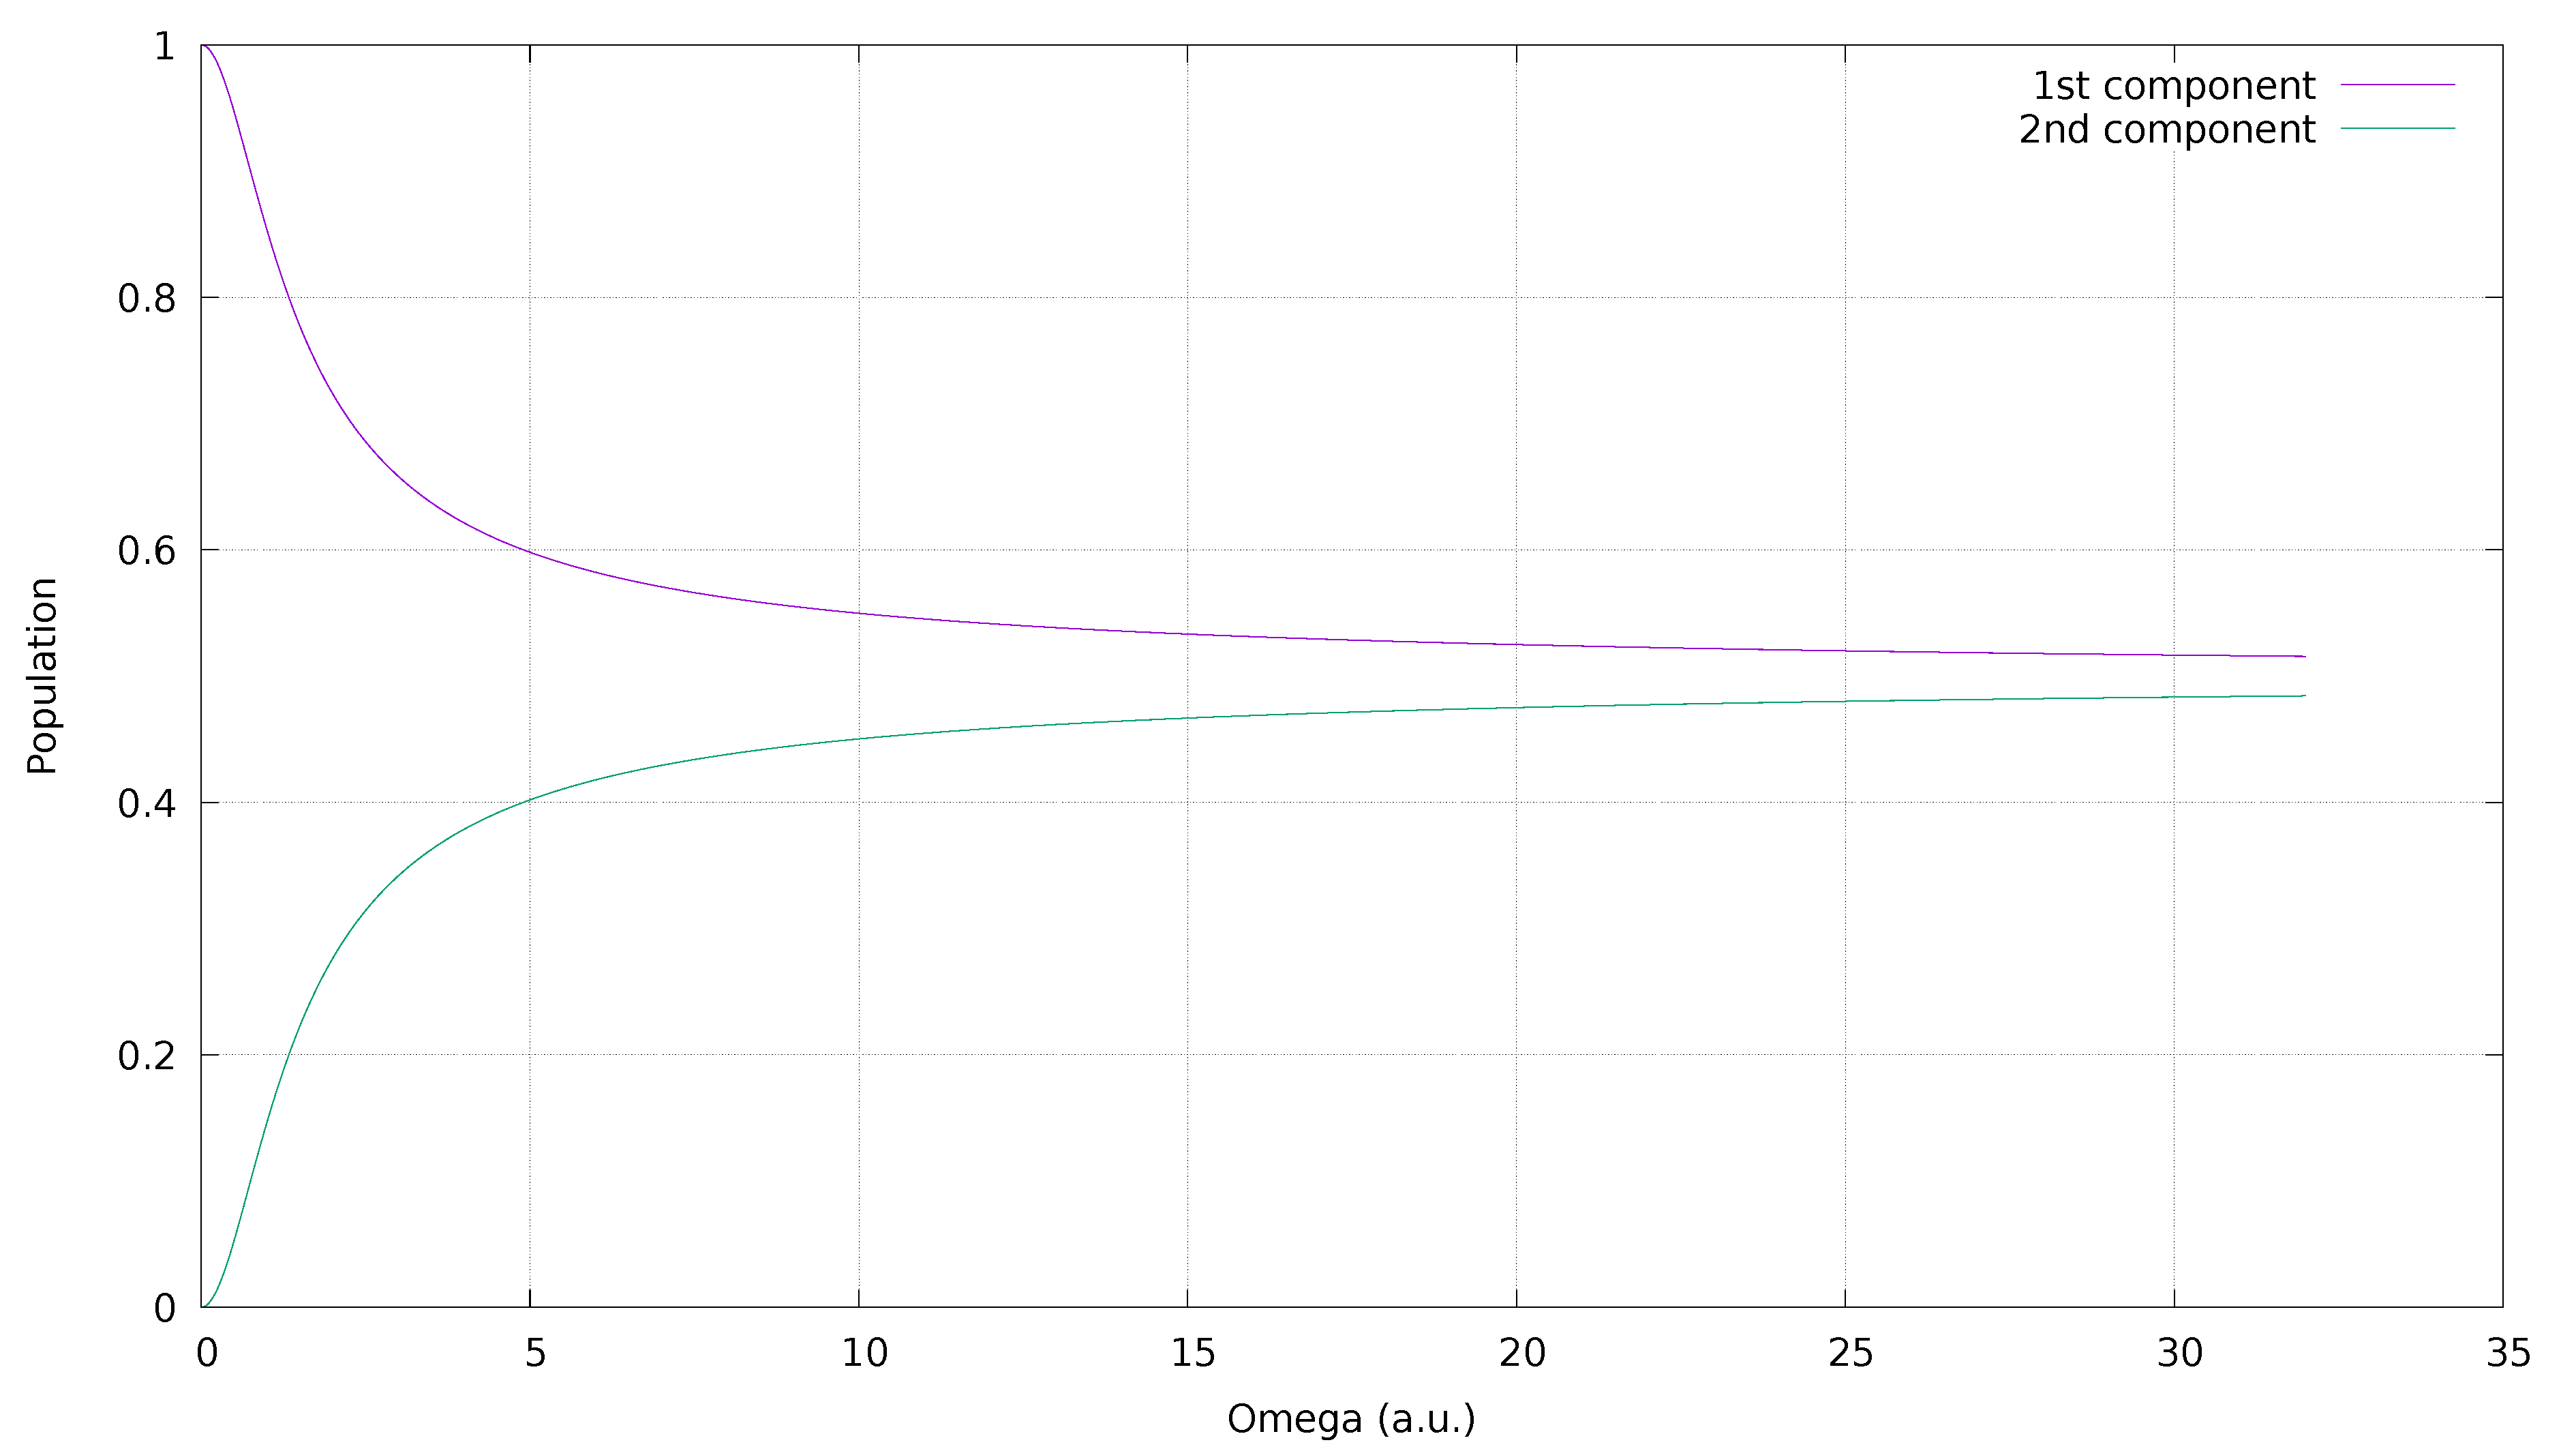
\includegraphics[width=.70\linewidth]{wavefunction_H2.pdf}
    \caption{Population of a 2 level atom interacting with laser fields according to $\Omega$}
    \label{fig:H2LVL}
\end{figure}
\newpage
and the 3 level one :
\begin{figure}[htbp]
    \centering
    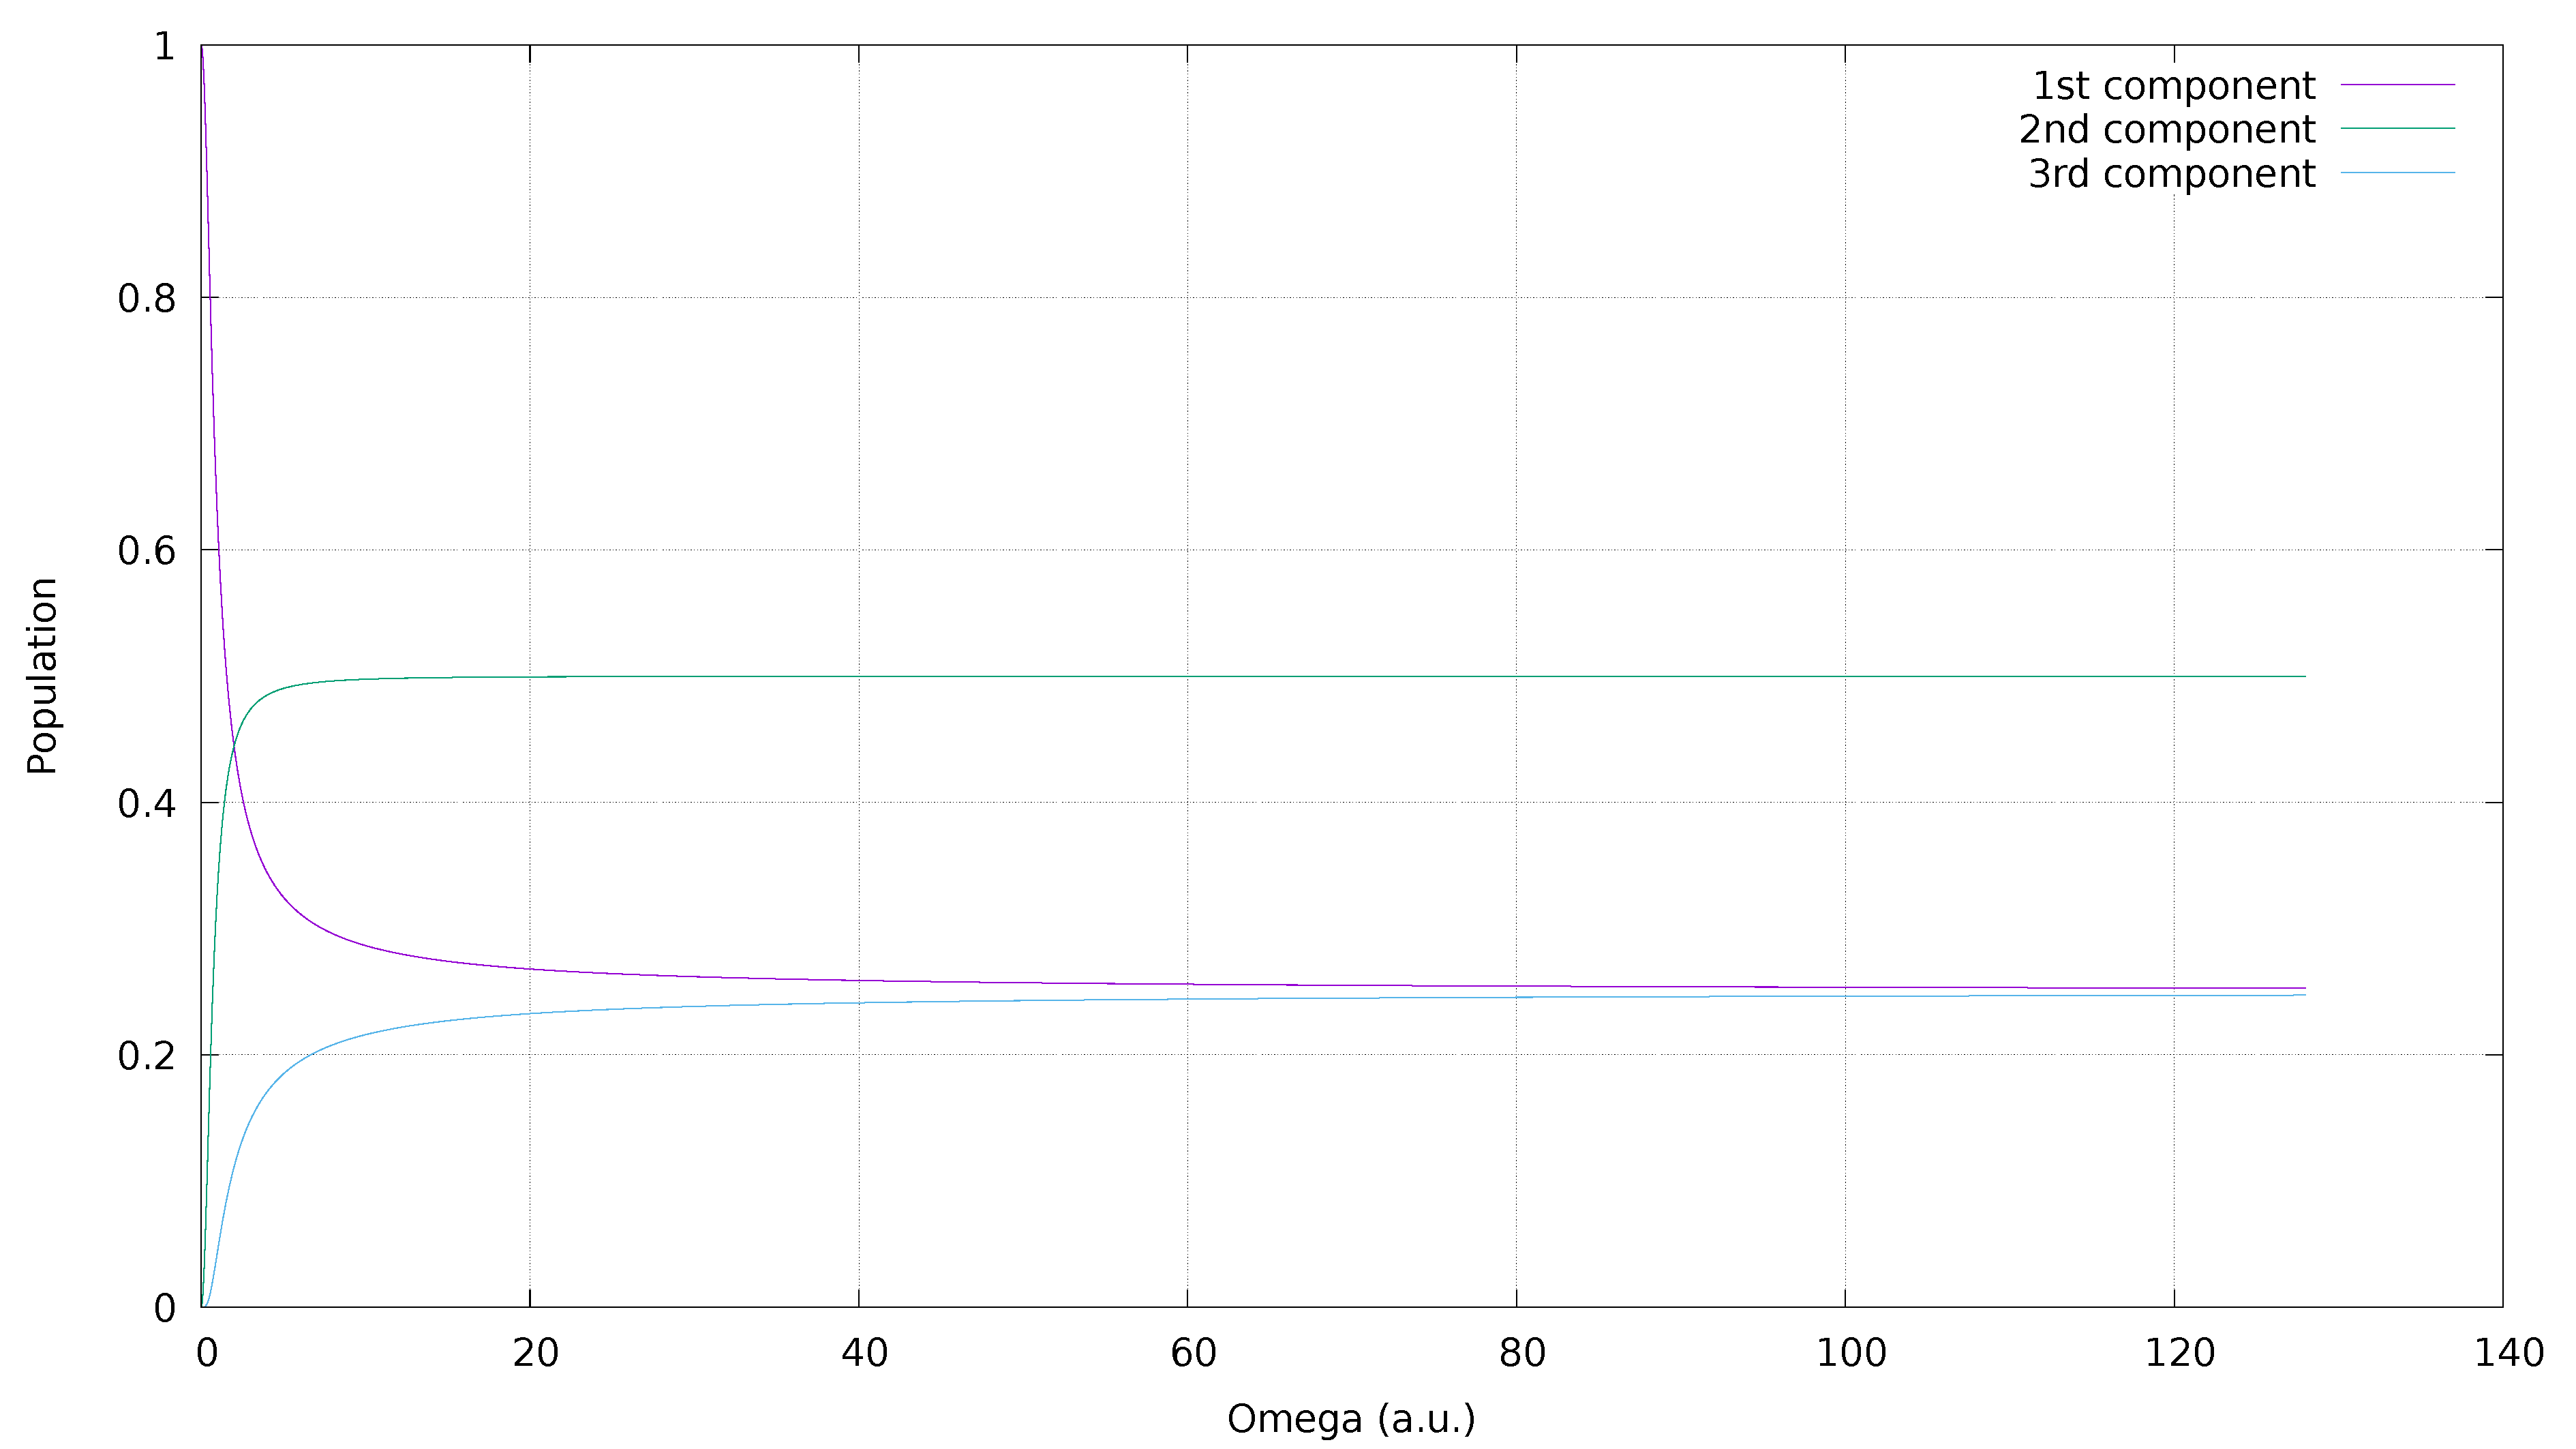
\includegraphics[width=.70\linewidth]{wavefunction_H3.pdf}
    \caption{Population of a 3 level atom interacting with laser fields according to $\Omega$}
    \label{fig:H3LVL}
\end{figure}\\
In the \autoref{fig:H2LVL}, we can see that all the population can by find onto the first level of the atom when there is no laser fields and none onto the second level. But when the amplitude of the laser field increase the first level lost population and the population goes onto the second level. Levels are stabilizing each other around $50\%$ of population for each level. For the \autoref{fig:H3LVL}, the levels 1 and 2 are acting like in the 2 level atom but they stabilize each other around $25\%$ of the population. But the third level gains $50\%$ of population for itself. So when you put a laser field onto an 3 level atom and increase its amplitude you will put half of the population onto the third level.\\
We have also draw the population of the molecular system according to $L$ (The size of the distribution of the potential) :
\begin{figure}[htbp]
    \centering
    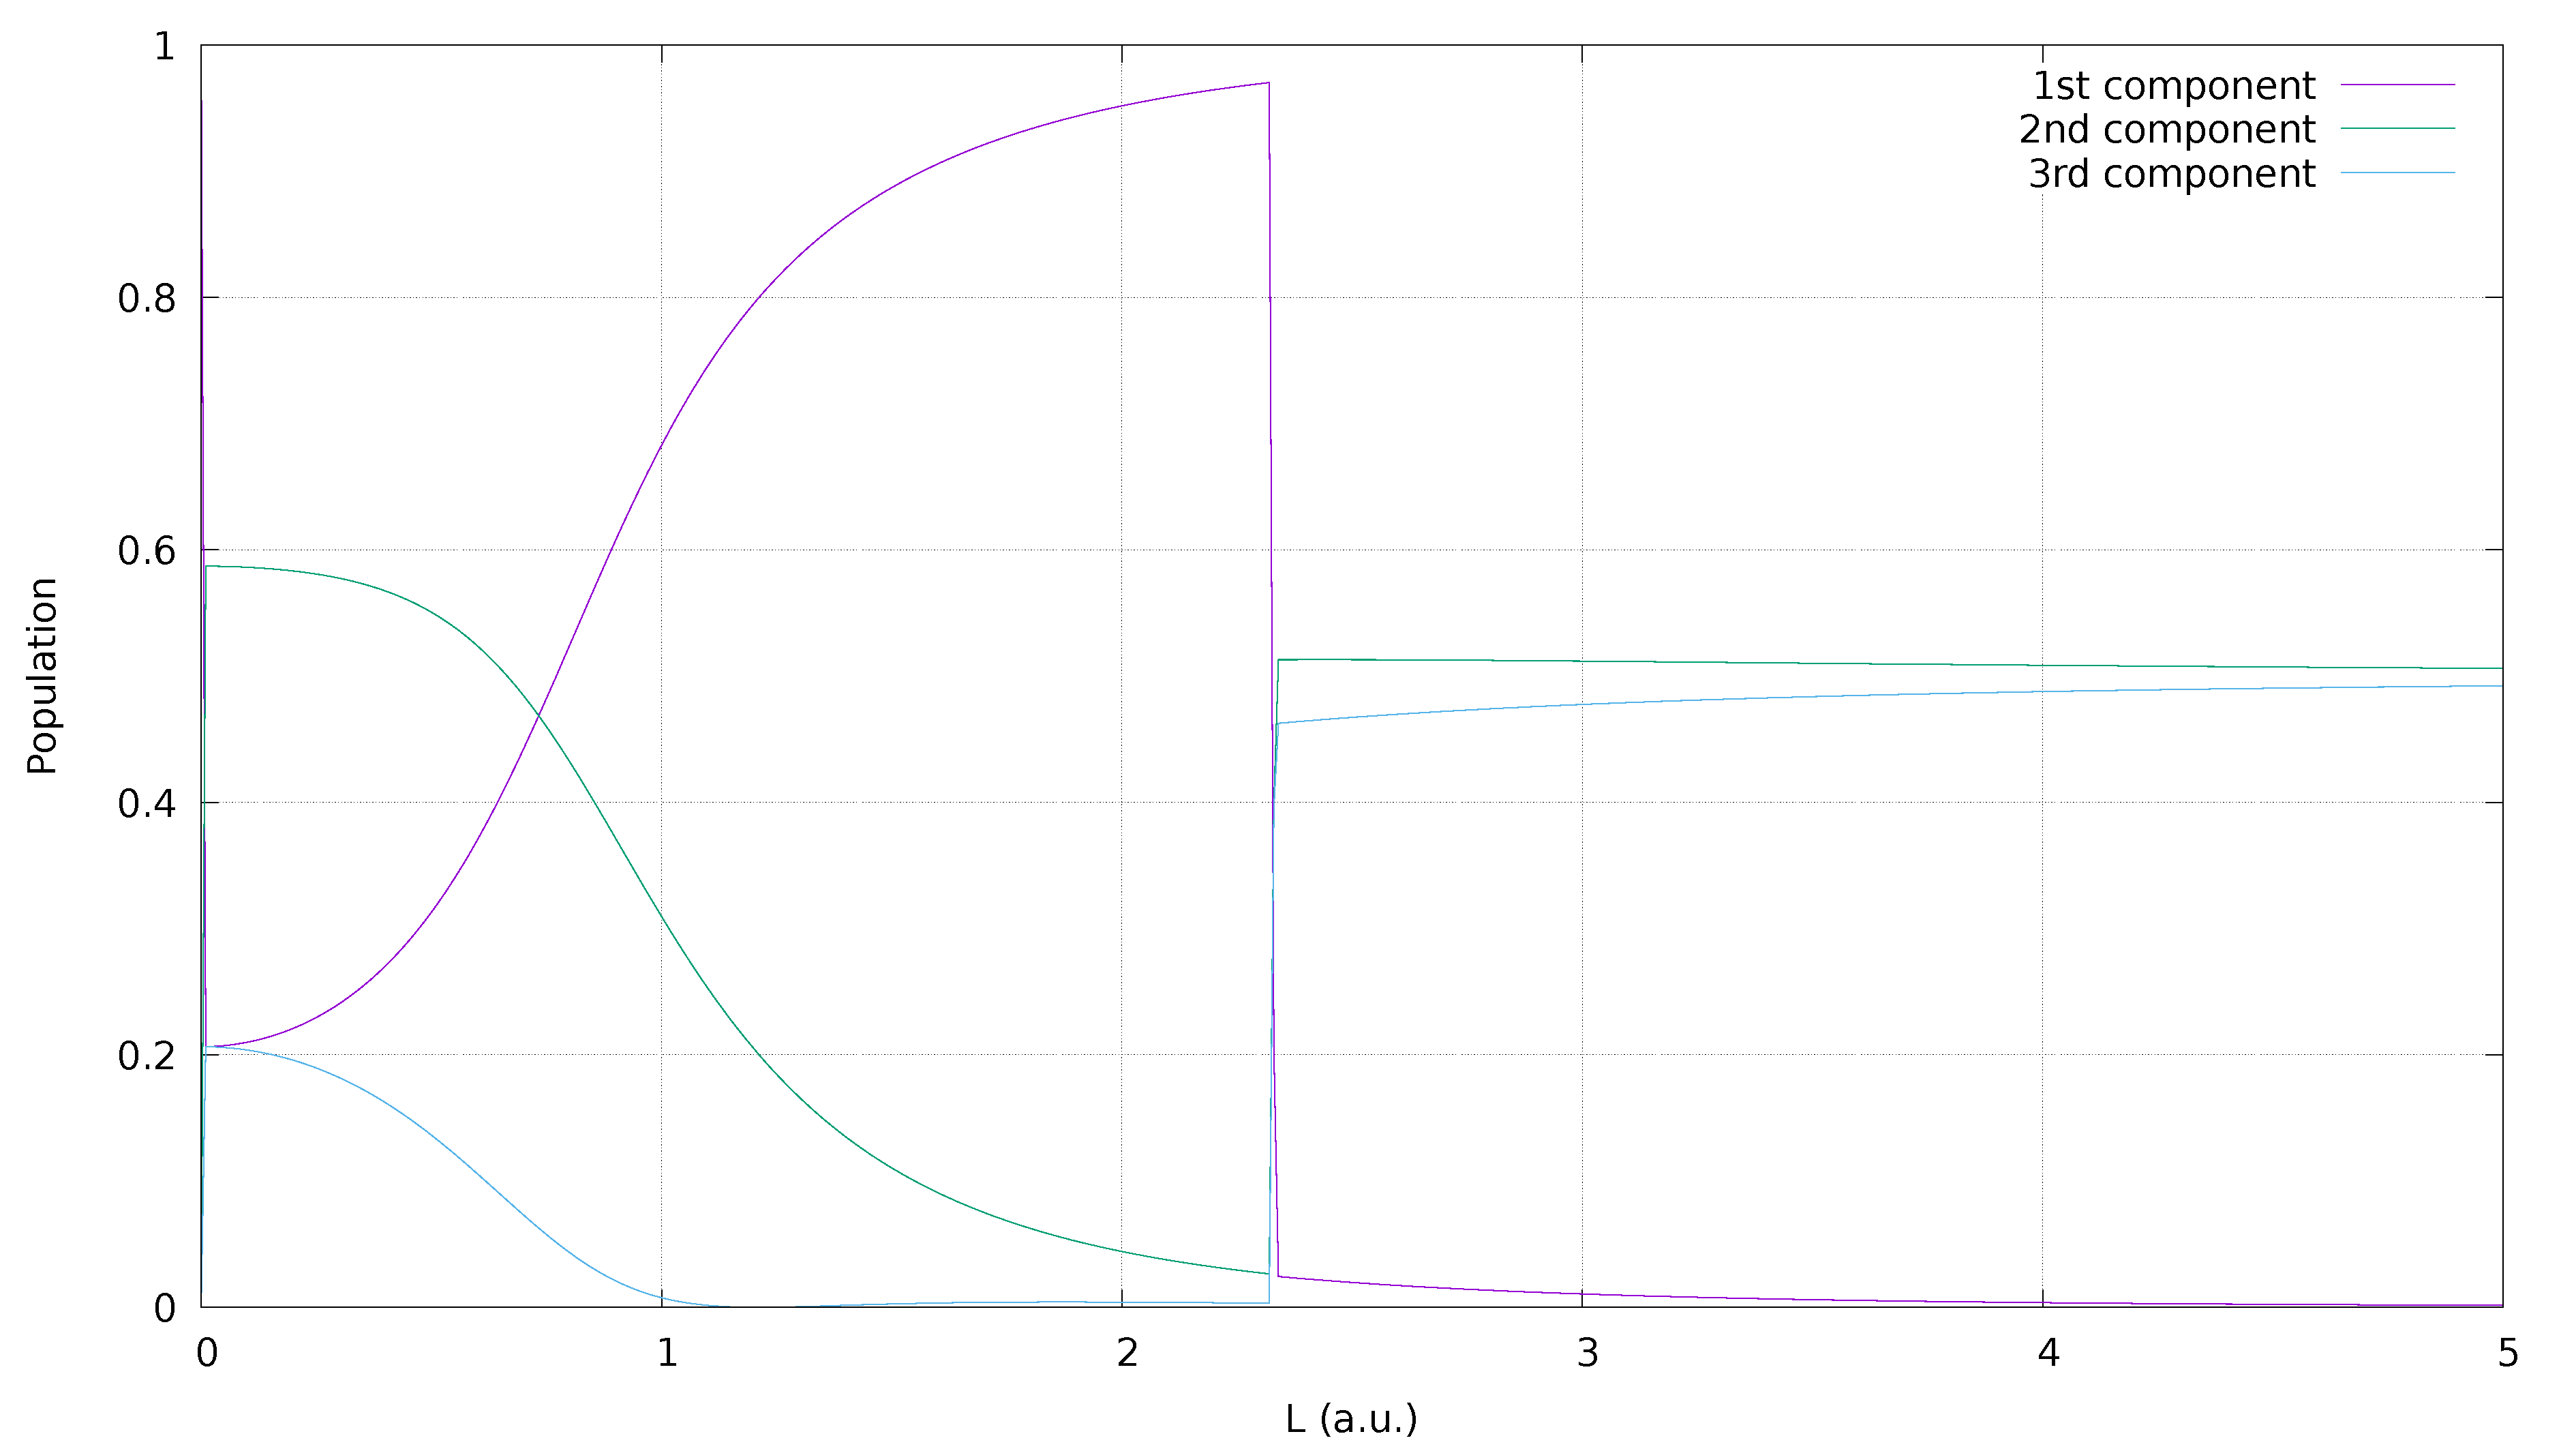
\includegraphics[width=.70\linewidth]{wavefunction_Hmol.pdf}
    \caption{Population of a molecular system according to $L$}
    \label{fig:H3LVL}
\end{figure}\\
We can see on the previous plot that when $L$ is null the population is at $60\%$ onto the third level and the other have $20\%$ of the population. But when $L$ increase the all the population goes to the first level then after a certain stade the population goes to level 2 and 3 and gave up the level 1. We can imagine that the distribution of the potential is too much big so it is easier for electrons/holes to move between atoms of the molecule.
\newpage
\section{Conclusion}
\label{sec:conclusion}
\noindent
This program can be usefull to find the ground state of an Hmiltonian. Unfortunately it is only working with the power iterative method. By correcting the Lanczos method the program could be improved because theoritically this method converge faster than the first one. To work on this project was a good opportunity to learn more about the diagonalization methods, even if the Lanczos one is a failure. But you can create your own Hamiltonian and compute its ground state easily.  
\newpage
\section{Appendix}
\label{app:app}
\subsection{Proof of the relation for the caracteristic polynomial}
\label{app:pol}
This proof will be done by induction.\\
We have :
\begin{equation}
    \begin{aligned}
        p_0(\lambda) &= 1\\
        p_1(\lambda) &= \alpha_0-\lambda_0\\
    \end{aligned}
\end{equation}
And we want to prove the statement, $S(k)$ :
\begin{equation}
    p_k(\lambda) = (\alpha_{k-1}-\lambda)p_{k-1}(\lambda)-|\beta_{k-1}|^2p_{k-2}(\lambda)\quad\forall k\in\{2,\hdots,n\}
\end{equation}
\\
\underline{Base case :}\\
For $k=2$ :
\begin{equation}
    \begin{aligned}
            p_2(\lambda) = \left|\begin{matrix}
                                \alpha_0 - \lambda & \bar{\beta}_1\\
                                \beta_1 & \alpha_1 - \lambda
                            \end{matrix}\right| &= (\alpha_0-\lambda)(\alpha_1-\lambda) - |\beta_{k-2}|^2\\
                                                &= (\alpha_0-\lambda)(\alpha_1-\lambda) - |\beta_{k-2}|^2\times 1\\
                                                &= (\alpha_0-\lambda)p_1(\lambda) - |\beta_{k-2}|^2p_0(\lambda)\\
    \end{aligned}
\end{equation}
So the statement is true for $k=2$.\\
\\
\underline{Inductive step :}\\
We suppose that, for $k>2$, $S(k)$ and $S(k-1)$ are true.
\begin{equation}
    \begin{aligned}
        p_{k+1}(\lambda) &= \left|\begin{matrix}
                    \alpha_0-\lambda & \bar{\beta}_1 & & 0\\
                    \beta_1 & \alpha_1-\lambda & \ddots & \\
                        & \ddots & \ddots & \bar{\beta}_{k}\\
                    0 & & \beta_{k} & \alpha_{k}-\lambda
                  \end{matrix}\right|\\
                &= (-1)^{2k+1}\beta_k\left|\begin{matrix}
                                        \alpha_0-\lambda & \bar{\beta}_1 & & 0\\
                                        \beta_1 & \alpha_1-\lambda & \ddots & \\
                                            & \ddots & \ddots & \\
                                        0 & & \beta_{k-1} & \bar{\beta}_{k}
                                      \end{matrix}\right| + (-1)^{2k+2}(\alpha_k-\lambda)\left|\begin{matrix}
                                                                                \alpha_0-\lambda & \bar{\beta}_1 & & 0\\
                                                                                \beta_1 & \alpha_1-\lambda & \ddots & \\
                                                                                    & \ddots & \ddots & \bar{\beta}_{k-1}\\
                                                                                0 & & \beta_{k-1} & \alpha_{k-1}-\lambda
                                                                              \end{matrix}\right|\\
                &= (-1)^{4k+1}|\beta_k|^2\left|\begin{matrix}
                        \alpha_0-\lambda & \bar{\beta}_1 & & 0\\
                        \beta_1 & \alpha_1-\lambda & \ddots & \\
                            & \ddots & \ddots & \bar{\beta}_{k-2}\\
                        0 & & \beta_{k-2} & \alpha_{k-2}-\lambda
                      \end{matrix}\right| + (-1)^{2k+2}(\alpha_k-\lambda)\left|\begin{matrix}
                                                                \alpha_0-\lambda & \bar{\beta}_1 & & 0\\
                                                                \beta_1 & \alpha_1-\lambda & \ddots & \\
                                                                    & \ddots & \ddots & \bar{\beta}_{k-1}\\
                                                                0 & & \beta_{k-1} & \alpha_{k-1}-\lambda
                                                              \end{matrix}\right|\\
                &= (\alpha_k-\lambda)p_k(\lambda)-|\beta_k|^2p_{k-1}(\lambda)
    \end{aligned}
\end{equation}
That is, the statement $S(k+1)$ also holds true, establishing the inductive step.\\
\\
\underline{Conclusion}\\
Since both the base case and the inductive step have been proved as true, by mathematical induction the statement $S(k)$ holds for every natural number $k$.

% \begin{table}[htbp]
%     \begin{center}
%         \begin{tabular}{p{0.3\linewidth} p{0.3\linewidth} p{0.3\linewidth}} \toprule
%             \multicolumn{3}{c}{\py{name}}\\
%             \midrule
%             \hfil Description & \hfil Input & \hfil Output\\
%             \cmidrule(r){1-1} \cmidrule{2-2} \cmidrule(l){3-3}
           
%             This function computes the Shannon entropy over time of $\theta$. So for each vector of the list of vectors \py{theta}&
            % \vspace*{-8pt}
            % \begin{itemize}[leftmargin=15pt, itemsep=0pt, topsep=0pt]
                % \setlength{\itemsep}{0pt}
                % \item \py{"random"}
                % \item \py{"chimera"}
                % \item \py{"inverse"}
                % \item \py{"josephson"}
                % \end{itemize}
%             &
%             This function will retrieve two data files in the parameters directory.
%             \begin{itemize}[leftmargin=15pt, itemsep=0pt, topsep=0pt]
%                 \item \py{"S.dat"} : It contains a list of real of size T. \py{S} represents the Shannon entropy over time of each vector of \py{theta}
%             \end{itemize}\\
%             \bottomrule
%         \end{tabular}
%     \end{center}
%     \caption{function}
%     \label{tab:label}
% \end{table}

% \begin{figure}[htbp]
%     \centering
%     \includegraphics[width=.95\linewidth]{../outcomes/josephson/phase.png}
%     \caption{Complex mean of phase josephson arrays}
%     \label{fig:phase_j}
% \end{figure}

% \newpage
% \bibliographystyle{plain}
% \bibliography{biblio}
\end{document}